\section{Detection and Segmentation}

\subsection{Overview}

计算机视觉中的四个典型任务：分类、语义分割、目标检测、实例分割。

\begin{figure}[H]
    \centering
    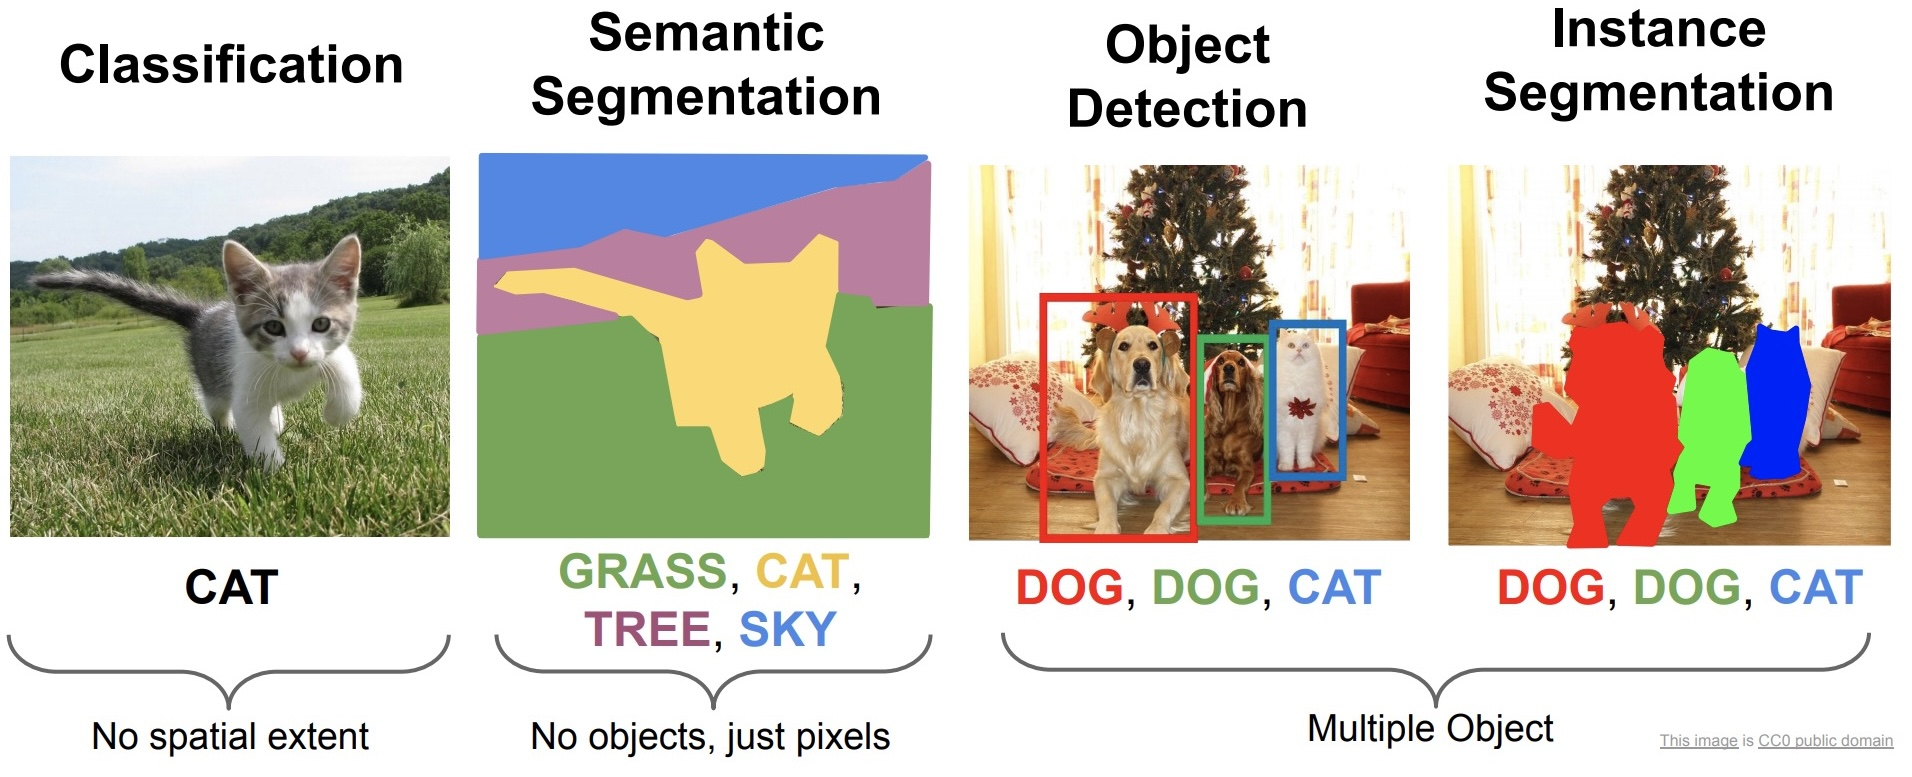
\includegraphics[width=0.8\linewidth]{figs/chapter6/cvtasks.jpg}
\end{figure}

\subsection{Semantic Segmentation}

对图像的每一个像素进行分类。

\paragraph{Idea 1: Sliding Window}

\begin{figure}[H]
    \centering
    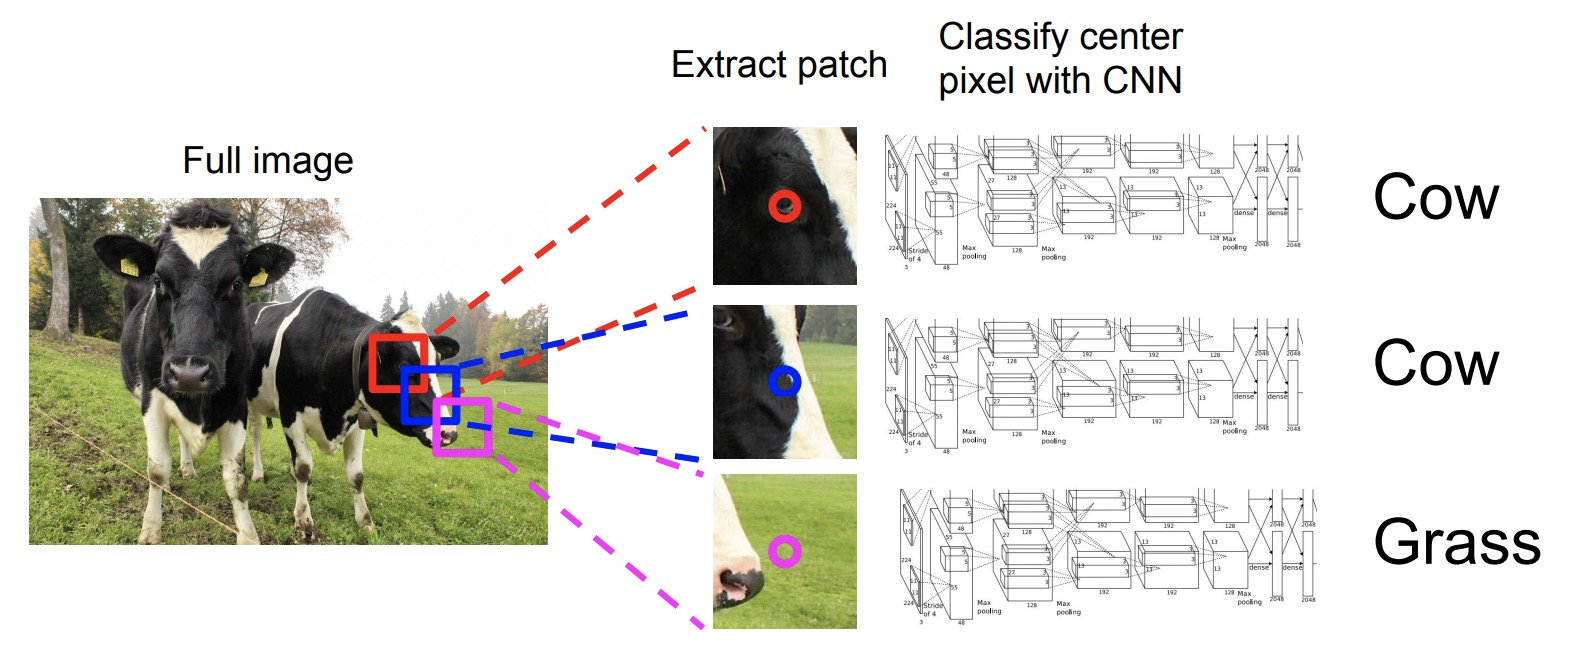
\includegraphics[width=0.8\linewidth]{figs/chapter6/slide.jpg}
\end{figure}

对每一个像素点用一个神经网络做一次分类。效率很差，进行了许多重复计算，nobody use it.

\paragraph{Idea 2: Fully Convolutional}

\begin{figure}[H]
    \centering
    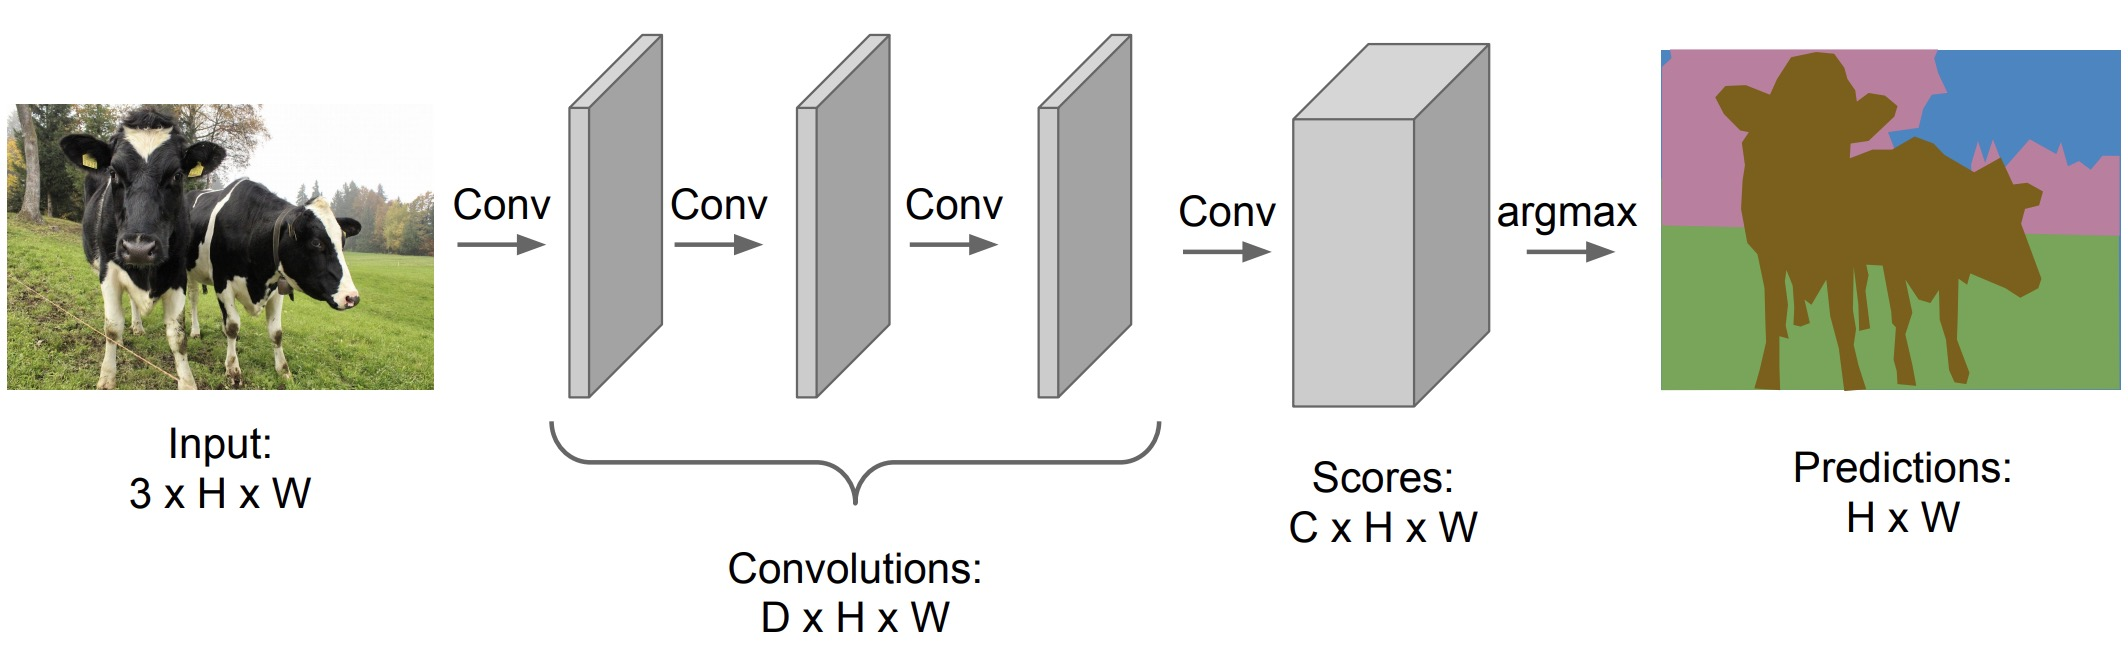
\includegraphics[width=0.8\linewidth]{figs/chapter6/fullyconv.jpg}
\end{figure}

经过一个卷积神经网络，每一个卷积层都\textbf{保持原图像的大小}，最终对每个像素都得到其各分类的得分，从而得到每个像素的分类结果。

问题：卷积非常耗时，因为每一个卷积层都保持原图像大小。

为了解决这个问题，我们可以先通过 $\text{max-pool}$ 或者 $\text{conv}$ 层进行 \textbf{downsampling}，然后再 \textbf{upsampling} 回原大小：

\begin{figure}[H]
    \centering
    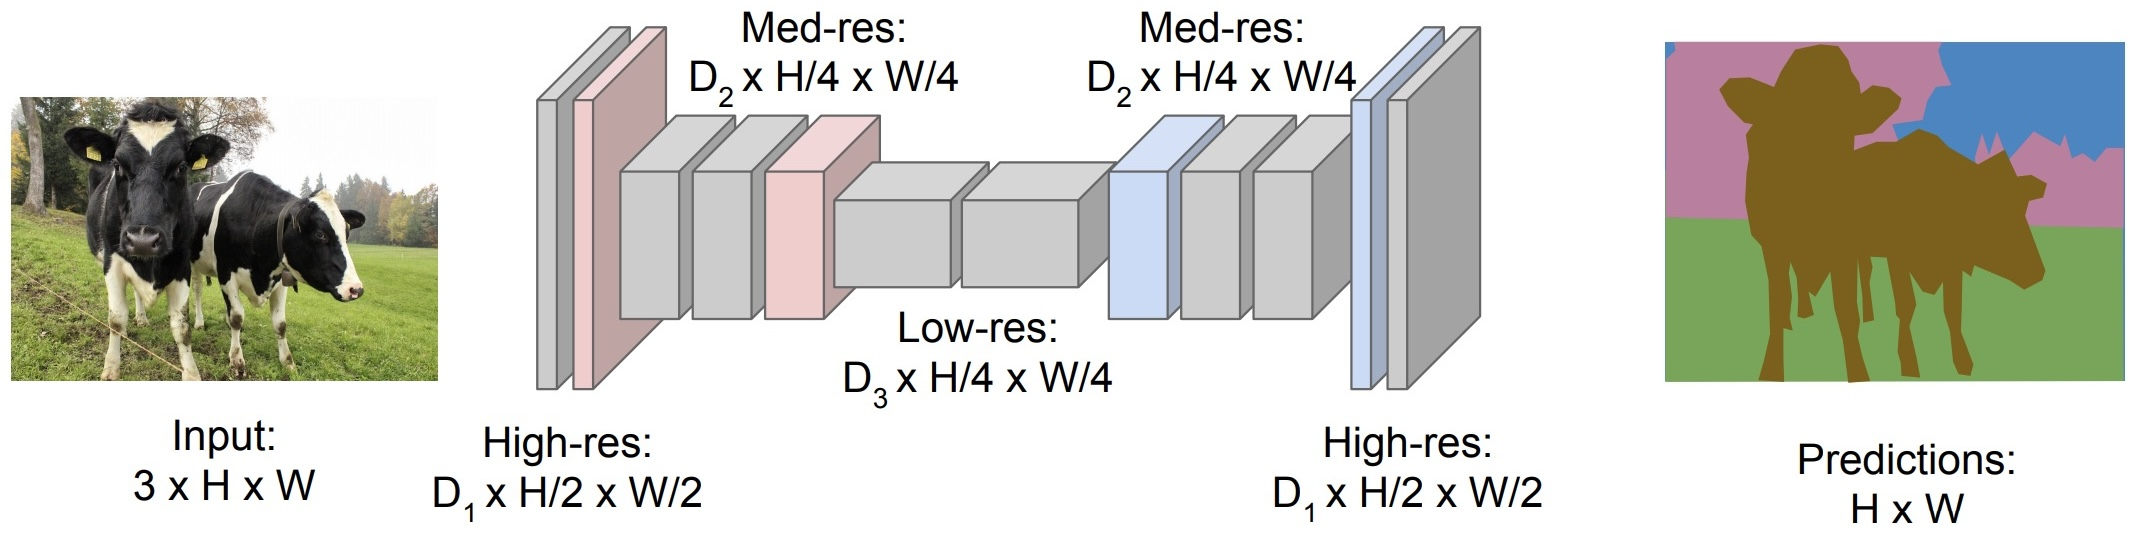
\includegraphics[width=0.8\linewidth]{figs/chapter6/fullyconv2.jpg}
\end{figure}

我们很清楚如何 downsampling，问题在于如何进行 \textbf{upsampling}：

\begin{itemize}
    \item \textbf{Unpooling}：

    \begin{figure}[H]
        \centering
        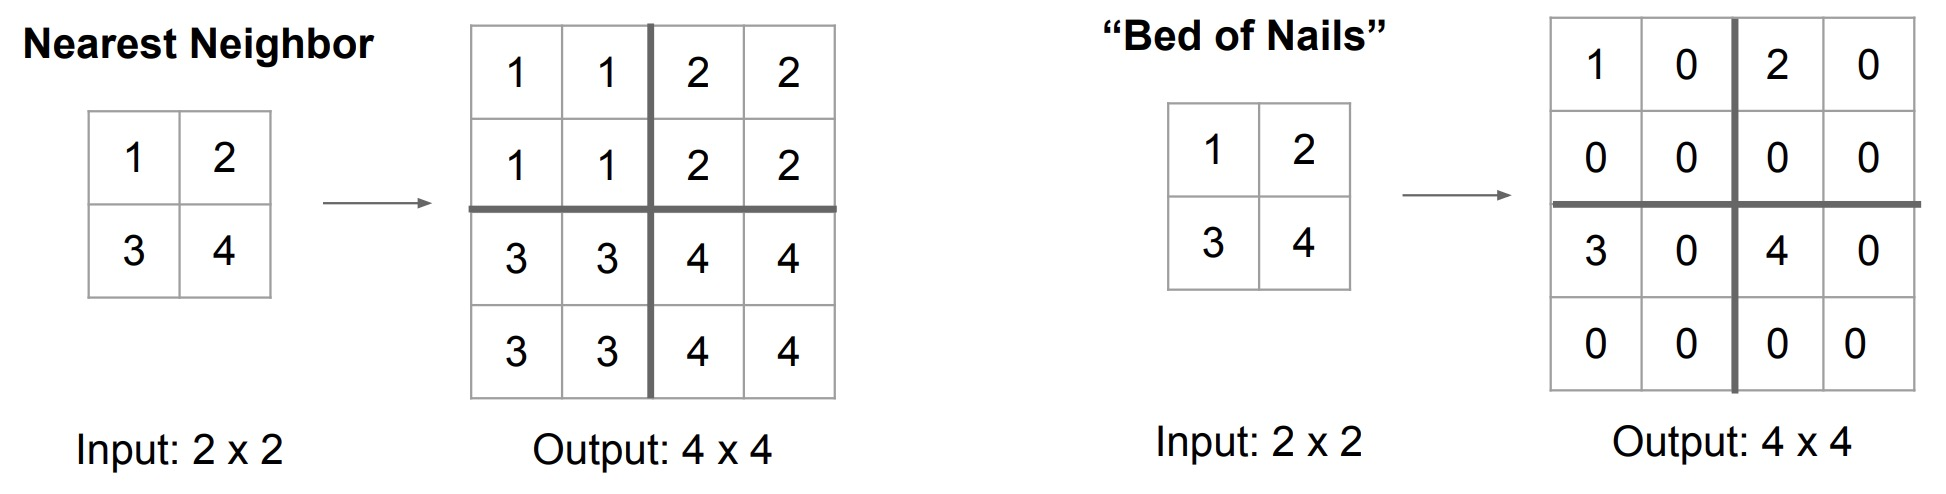
\includegraphics[width=0.8\linewidth]{figs/chapter6/unpooling.jpg}
    \end{figure}

    \item \textbf{Max-unpooling}：

    \begin{figure}[H]
        \centering
        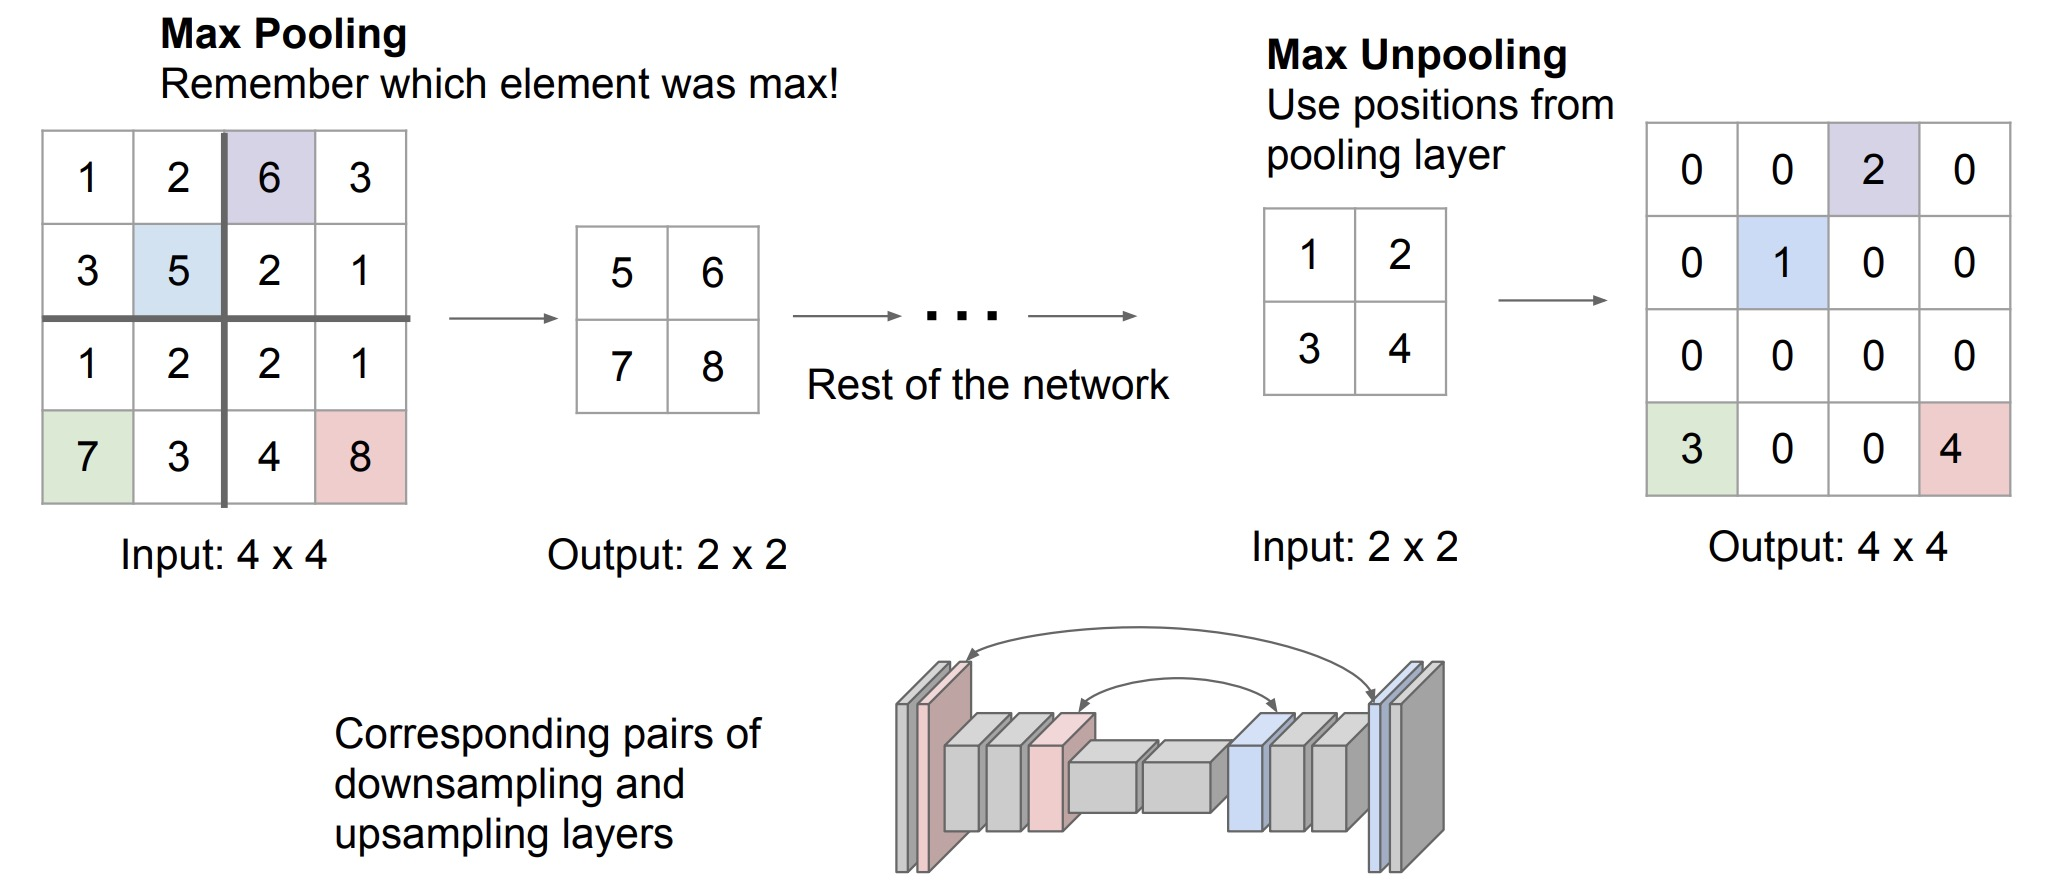
\includegraphics[width=0.8\linewidth]{figs/chapter6/maxunpooling.jpg}
    \end{figure}

    \item \textbf{Transpose Convolution}：

    视输入矩阵为 filter 的权重，按权重将 filter 累加到输出矩阵中。

    \begin{figure}[H]
        \centering
        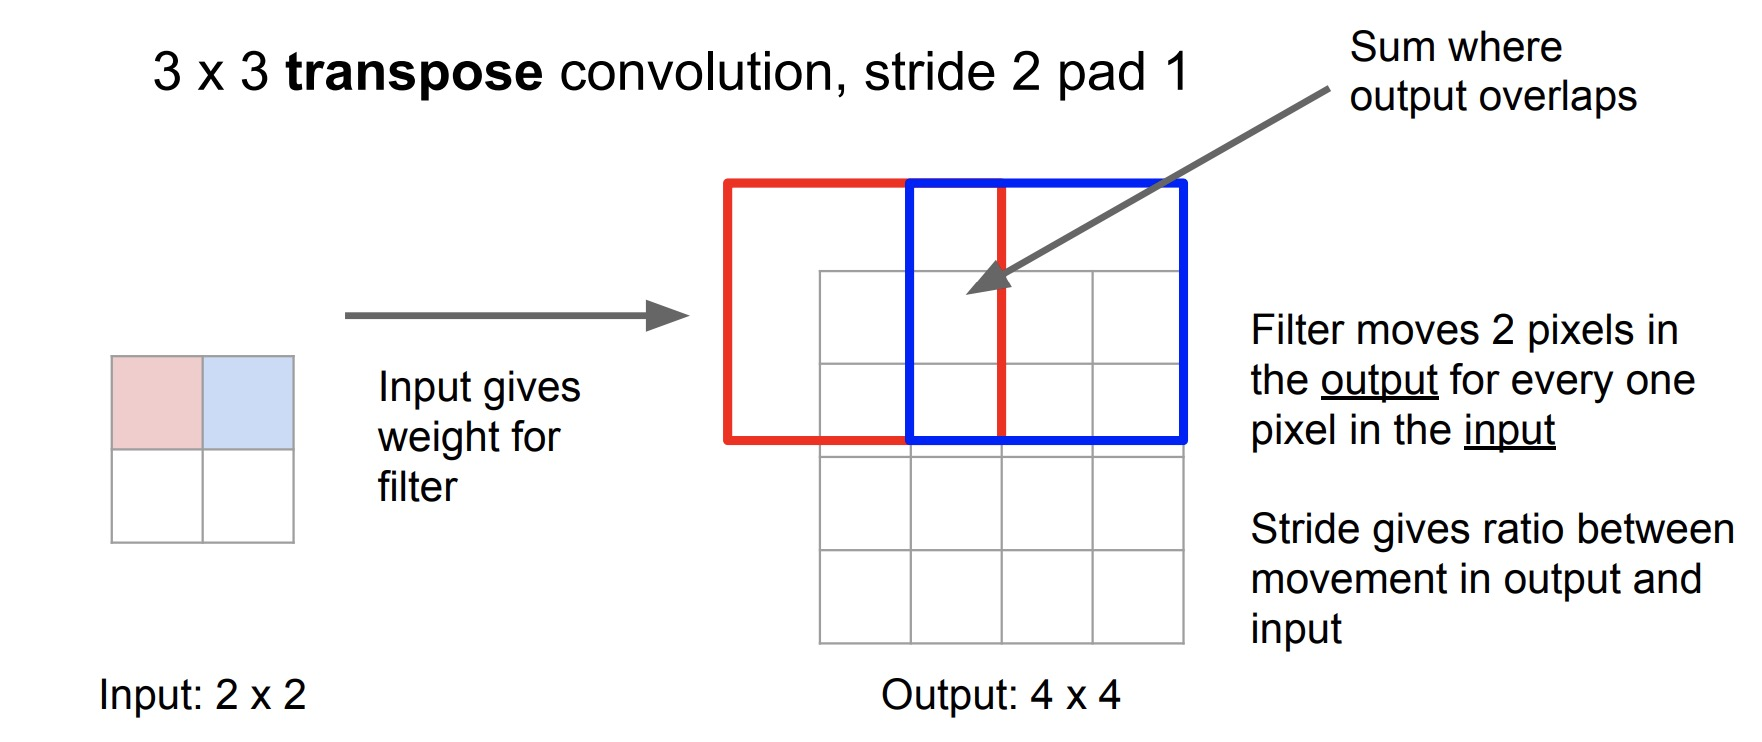
\includegraphics[width=0.8\linewidth]{figs/chapter6/transconv.jpg}
    \end{figure}

    \textbf{Transpose Convolution} 只能恢复卷积前后的大小，并不能恢复值，其原理是：

    在 Convolution 操作时，我们可以将输入图像拉伸为 $1$ 维向量 $X\in\mathbb R^{D}$，输出图像拉伸为 $1$ 维向量 $Y\in\mathbb R^{D'}$，则卷积核可以写作一个稀疏矩阵 $C\in \mathbb R^{D'\times D}$，使得 $CX=Y$. 在 Upsampling 中，已知 $C,Y$，欲得到 $X$，Transpose Convolution 的操作是：$X=C^TY$，这也是其名称的由来。显然这样做并没有恢复值，除非 $CC^T=I$.

\end{itemize}

\subsection{Object Detection}

\paragraph{Idea 1: Regression}

构造神经网络输出检测物体的类别以及框住物体的矩形框的坐标 $(x,y)$ 和大小 $(w,h)$.

由于在 Object Detection 中，我们并不能实现知道输入图像中有多少个 object，所以其输出大小是不固定的，并且当 object 很多时输出将很大。因此这不是一个很好的方法。

\paragraph{Idea2: Sliding Window}

滑动一个矩形框，每次对矩形框内的图像进行分类。

\begin{figure}[H]
    \centering
    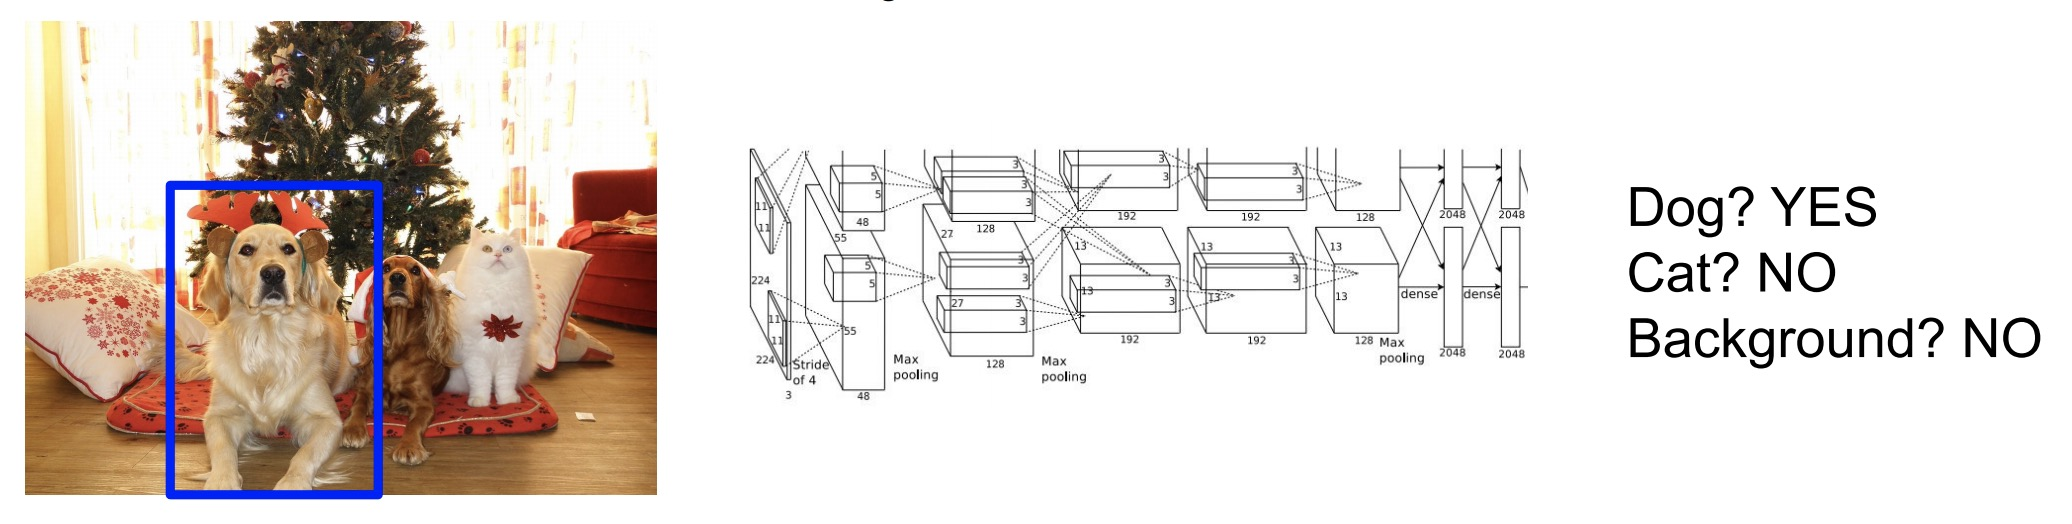
\includegraphics[width=0.8\linewidth]{figs/chapter6/obde_sliding.jpg}
\end{figure}

该方法也有很明显的问题：矩形框的位置和大小都是未知的，我们需要暴力遍历各种矩形框，每次都通过一个巨大的 CNN 网络得到类别，这无疑十分耗时。

\paragraph{Idea 3: Region Proposals \& R-CNN}

\begin{itemize}
    \item \textbf{Region Proposals}: 先通过一个网络给出物体可能存在的若干矩形范围，后续工作只需在这些范围内进行。\textbf{Selective Search} 是一种给出 Region Proposals 的方法，其运行速度非常快。

    \item \textbf{R-CNN}：在每一个给定的矩形范围内，我们可以构建 CNN 网络，输出该矩形内物体的类别以及这个矩形区域应该如何修正。注意由于每个矩形大小不同，而我们的网络要求特定大小的输入，所以我们会先对这些矩形进行变形使之符合网络的输入要求。具体见下图：

    \begin{figure}[H]
        \centering
        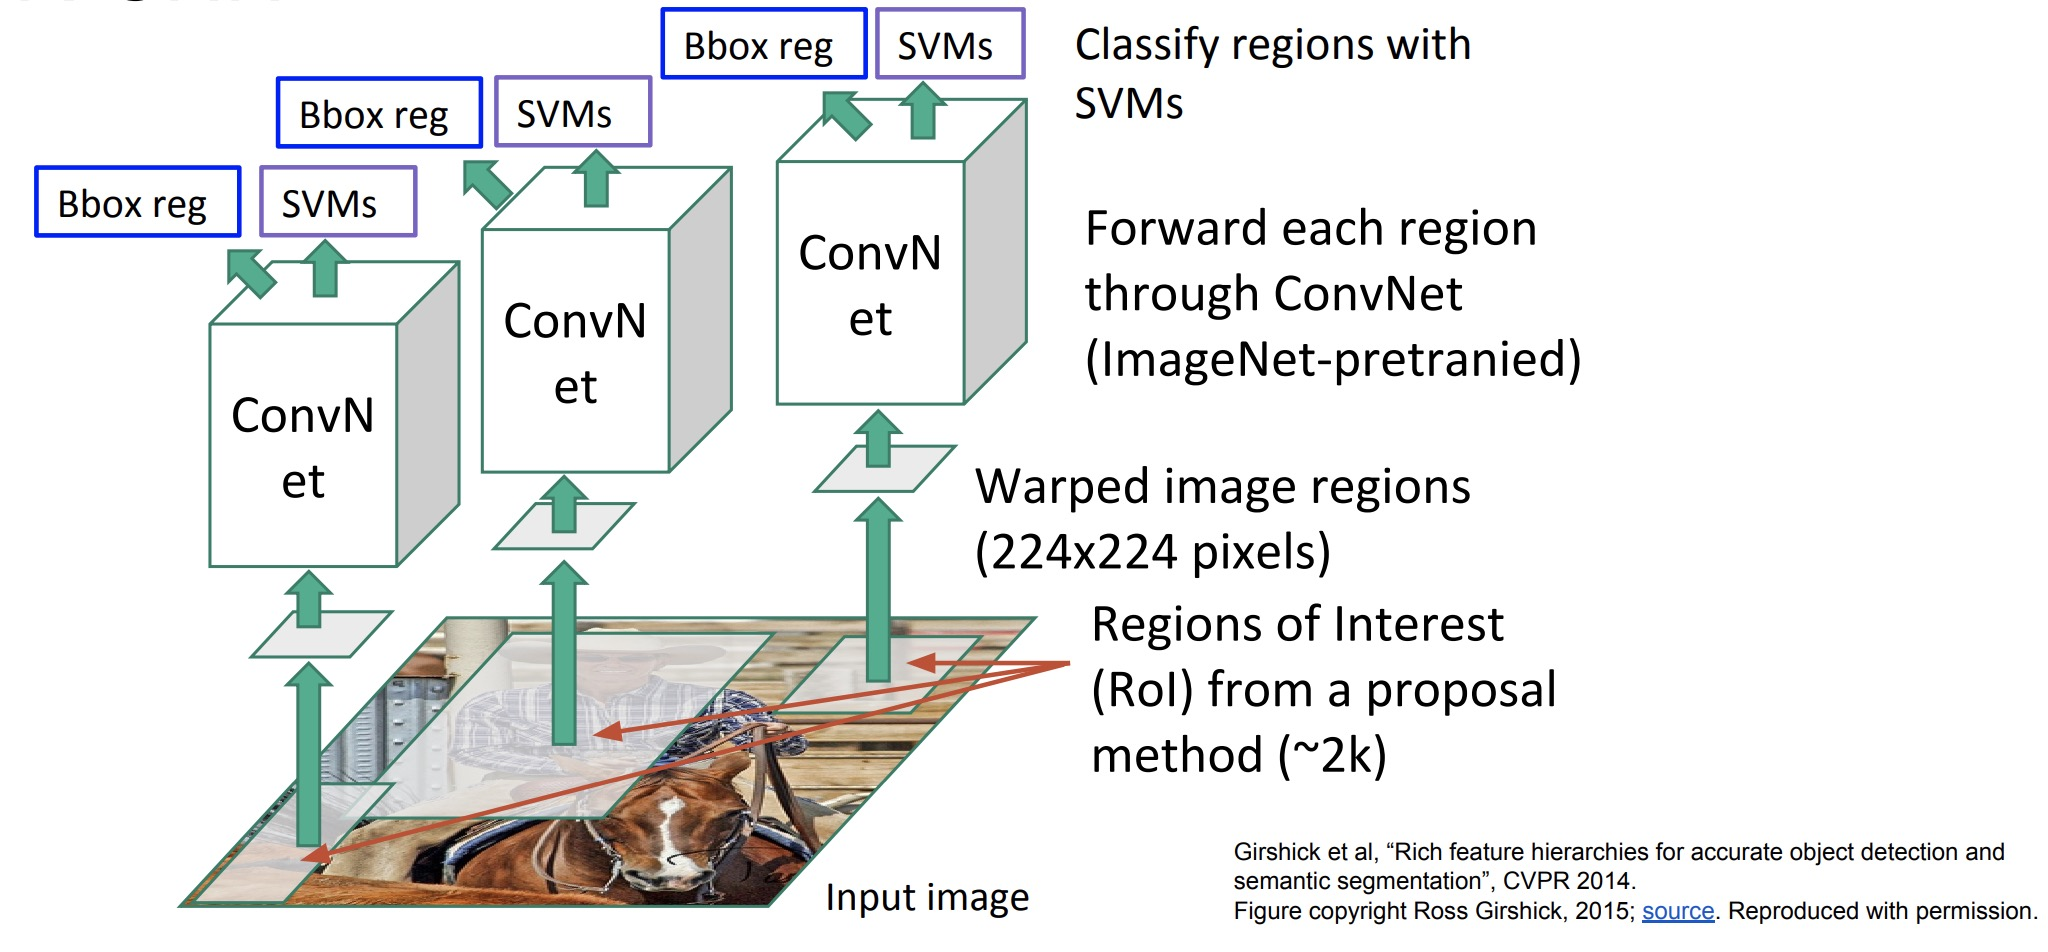
\includegraphics[width=0.8\linewidth]{figs/chapter6/R-CNN.jpg}
    \end{figure}

    该方法的不足在于，对每个矩形区域进行计算依然十分耗时耗力。

    \item \textbf{Fast R-CNN}：Idea 是我们先把图像输入进 CNN 网络，再对网络的输出结果进行矩形区域划分，这样图像只会经过一次 CNN 网络，从而提高运行速度。

    \begin{figure}[H]
        \centering
        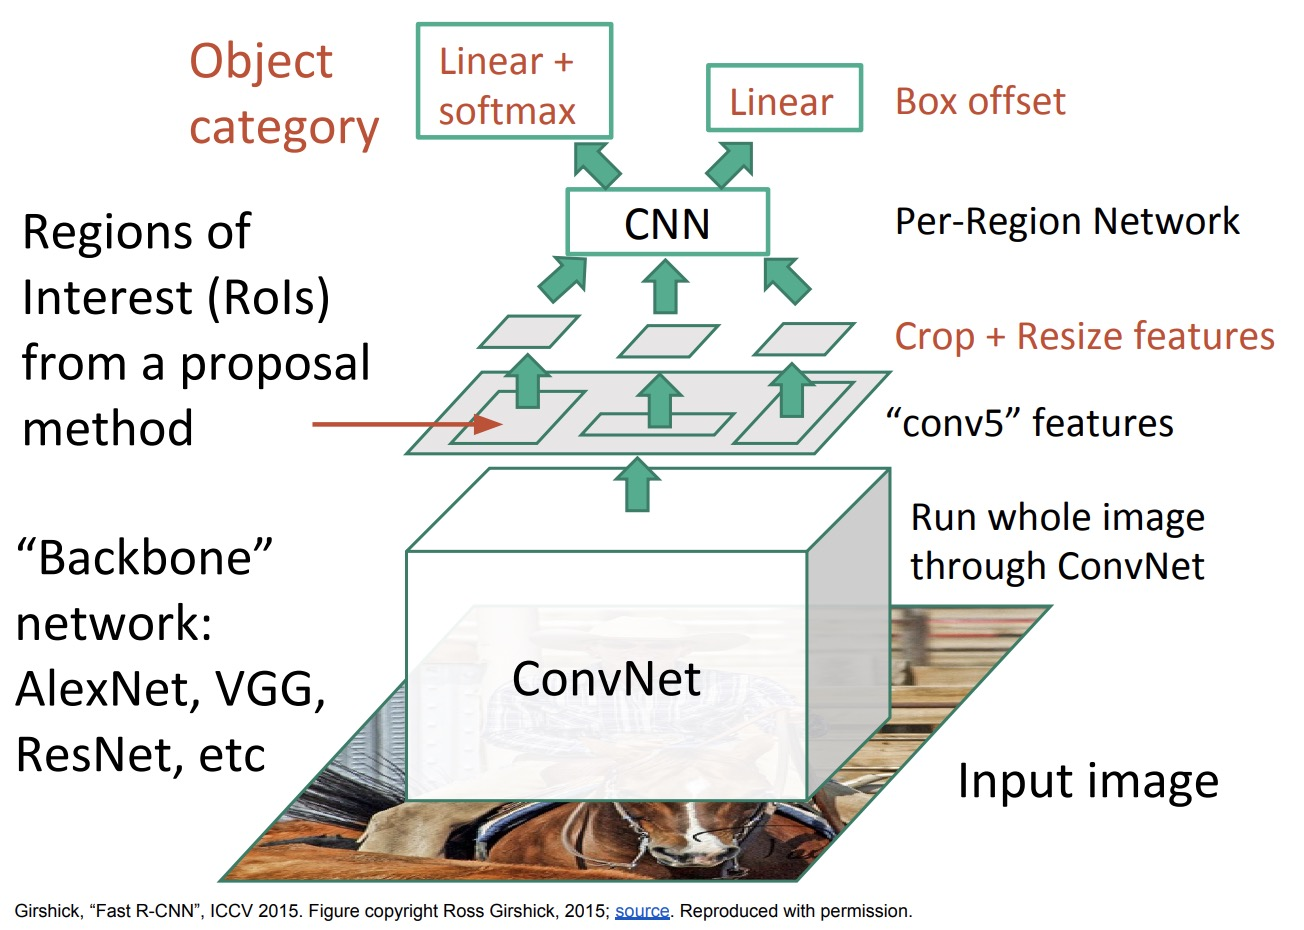
\includegraphics[width=0.6\linewidth]{figs/chapter6/Fast R-CNN.jpg}
    \end{figure}

    这里有个问题是如何在 CNN 网络的输出结果上进行 Region Proposals：

    \begin{itemize}
        \item \textbf{RoI (Region of Interest) Pool}：首先把原图像上的矩形区域按比例投影到输出矩阵上，然后取整使矩形端点落在整点上，对于这个矩形，我们将其尽可能地等分成需要的形状，并在每一块中作 $\text{max-pool}$，最终得到该区域的 feature.

        \begin{figure}[H]
            \centering
            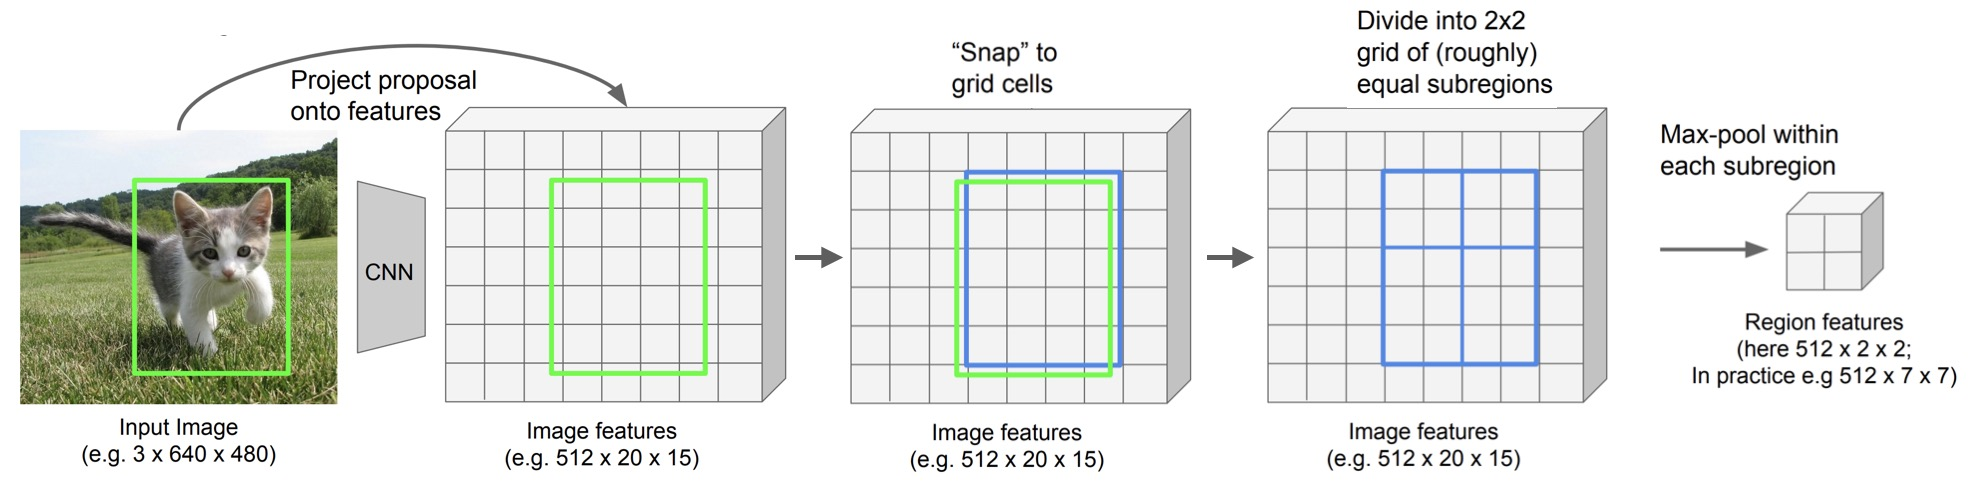
\includegraphics[width=1\linewidth]{figs/chapter6/RoI pool.jpg}
        \end{figure}

        由于我们在这个过程中进行了两次近似——取整和划分，所以这种方法的问题在于我们得到的区域特征稍有偏离。

        \item \textbf{RoI Align}：仍然把原图像上的矩形区域投影到输出矩阵上，然后直接等距离划分成需要的形状；现在考察每一个小块，它们的顶点不一定在整点上，我们在其中取 $4$ 个位置，对每个位置用它周围的 $4$ 个整点的值作双线性插值，然后取 $\text{max-pool}$，最终得到该区域的 feature.

        \begin{figure}[H]
            \centering
            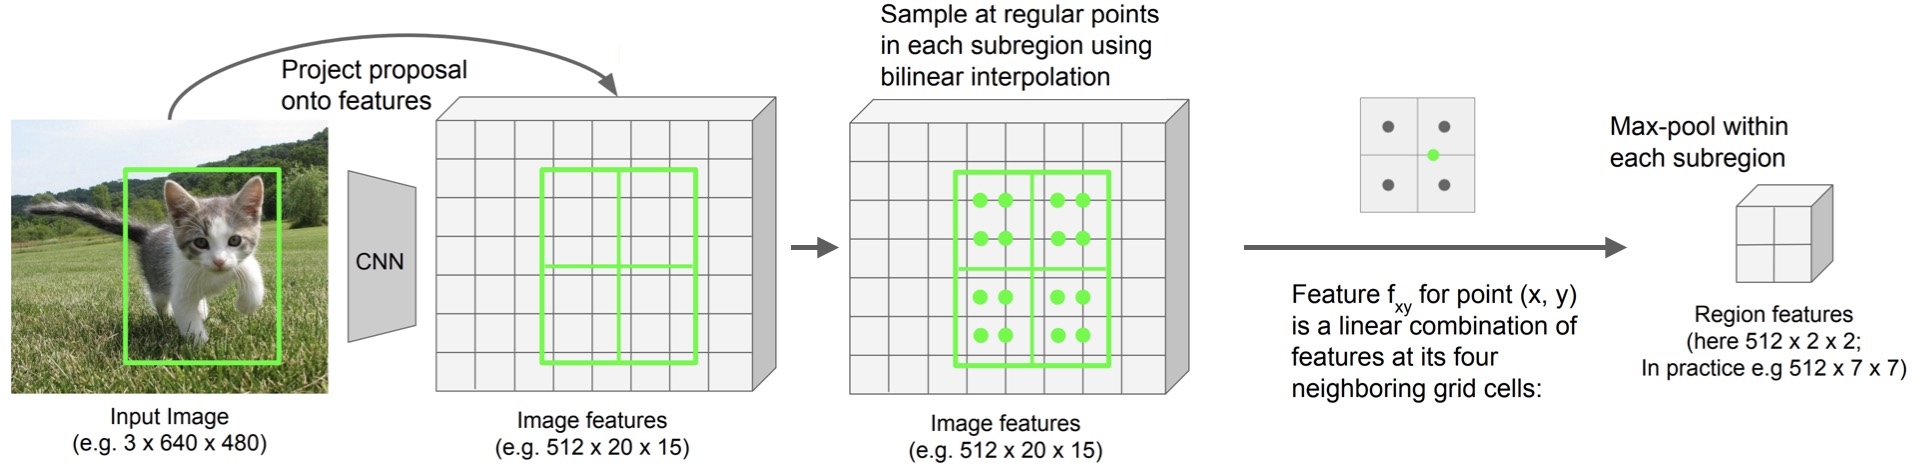
\includegraphics[width=1\linewidth]{figs/chapter6/RoI align.jpg}
        \end{figure}
    \end{itemize}

    \item \textbf{Faster R-CNN}：实测中发现，在 Fast R-CNN 中，Region Proposals 占了大部分时间。为了提高这部分的速度，Faster R-CNN 用一个 \textbf{Region Proposal Network} 在 CNN 的输出矩阵上作矩形区域划分，其余部分和 Fast R-CNN 相同。

    \begin{figure}[H]
        \centering
        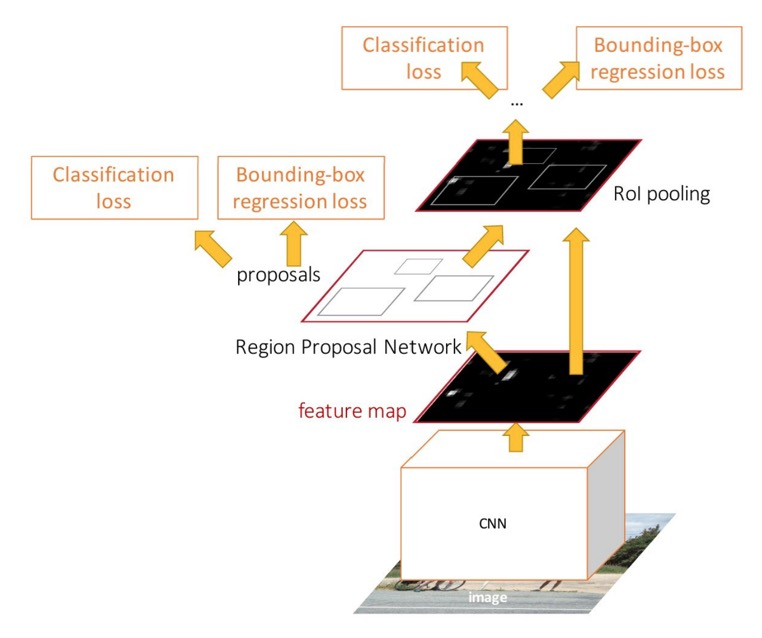
\includegraphics[width=0.5\linewidth]{figs/chapter6/Faster R-CNN.jpg}
    \end{figure}

    Region Proposal Network (RPN) 的原理如下：

    \begin{enumerate}
        \item 想象以 feature map 的每一个位置为中心有固定大小的 anchor box，使用一个 CNN 预测这些 anchor box 中是否有物体，以及对 box 四边的修正值。
        \item 对于每一个位置，计算 $K$ 个不同的 anchor box，这样我们得到了 $K\times H\times W$ 个数值表示该 anchor 处是否有物体，以及 $4K\times H\times W$ 个数值表示 box 四边的修正值。
        \item 取得分最高的约 $300$ 个 anchor box 作为我们的 region proposals.
    \end{enumerate}

    \begin{figure}[H]
        \centering
        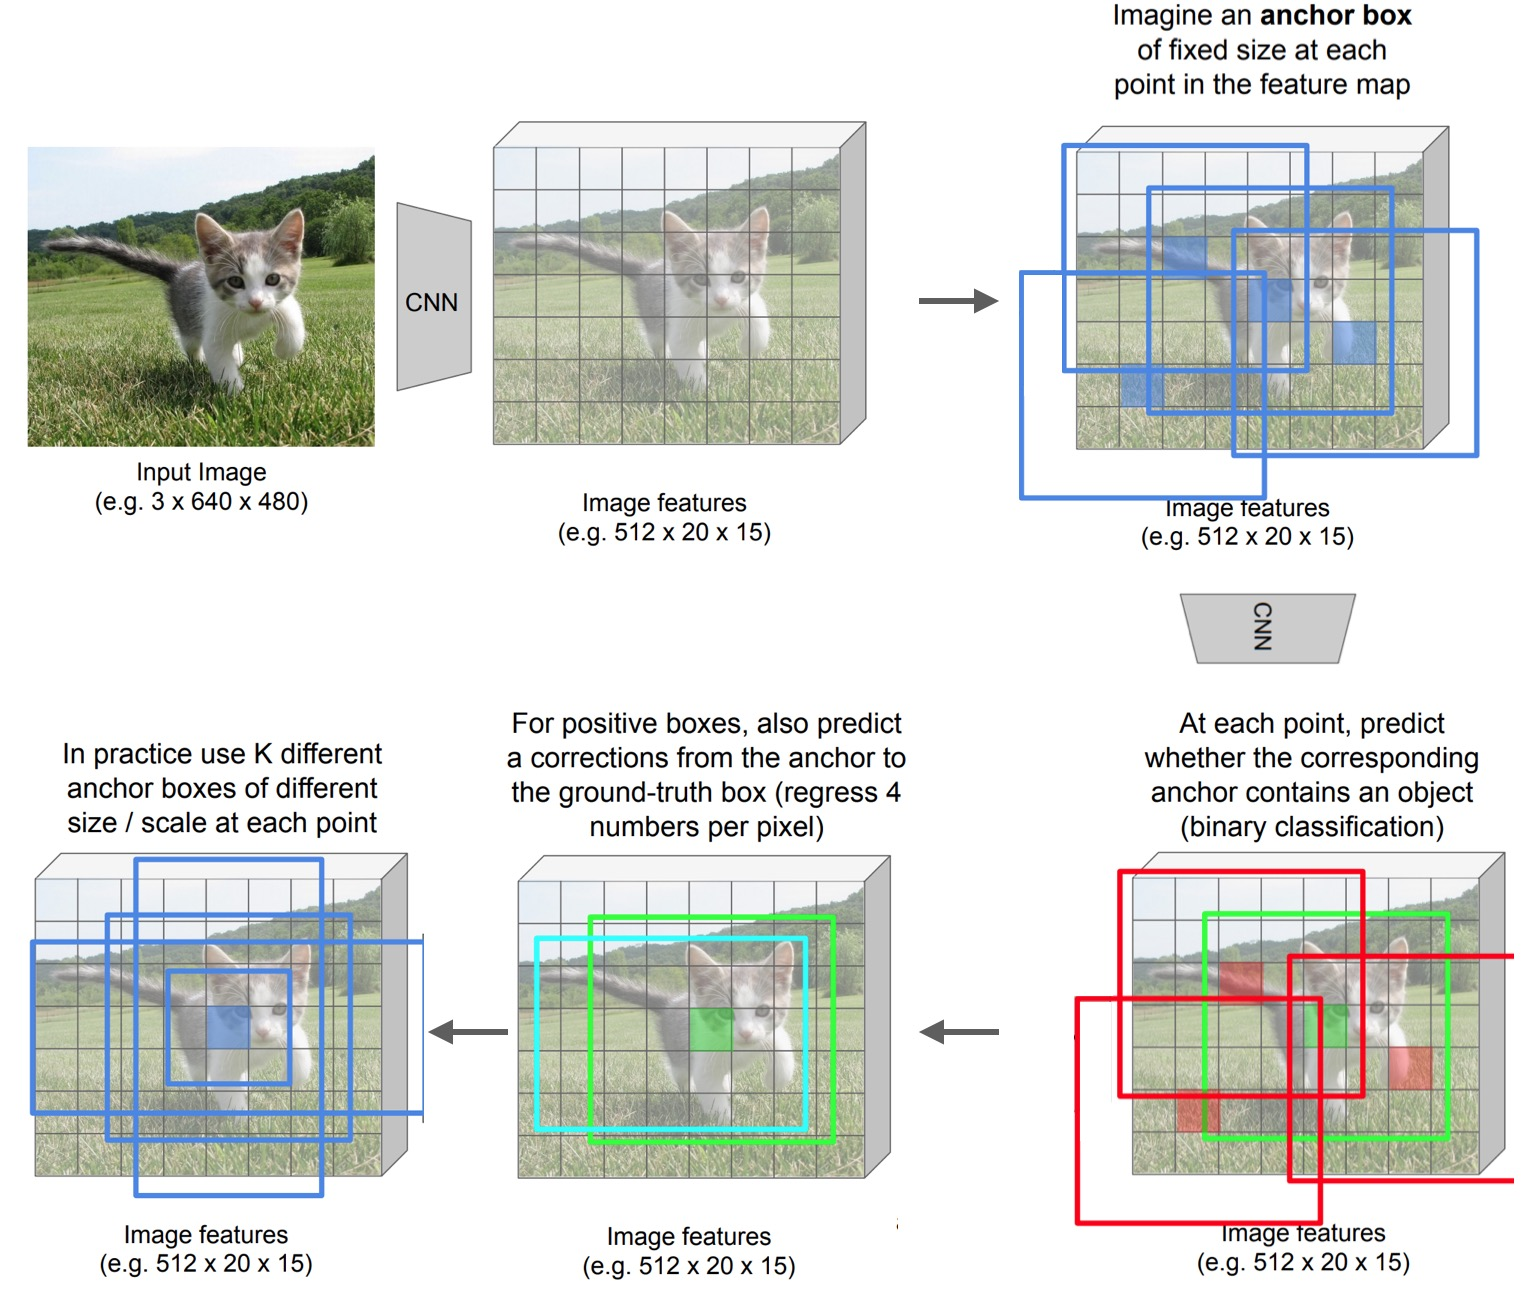
\includegraphics[width=0.9\linewidth]{figs/chapter6/RPN.jpg}
    \end{figure}

    在训练时，我们会将四个 loss 一起训练—— RPN 二分类（判断是否是物体）、RPN anchor box 位置的 loss、最终分类（判断是何物）的 loss、最终 box 的坐标的 loss.

    \item \textbf{YOLO / SSD / RetinaNet}：Faster R-CNN 其实有两个阶段：第一个阶段是得到 region proposals，通过一个基础的 CNN 和 RPN 完成，第二个阶段是对每一个 region 进行分类以及修正边界，通过 RoI pool / align 之后输入到 CNN 完成。而 YOLO / SSD / RetinaNet 等网络只用一个阶段，具体的内容不在此课程中讲授。

\end{itemize}

可以看出，Object Detection 有很多选择：首先，基础的网络有很多选择（VGG16 / ResNet-101 / Inception V2……）；接下来，我们可以选择二阶段的 Faster R-CNN 或者单阶段的 YOLO / SSD 或者混合的 R-FCN……这其中就有许多的 trade-offs. 例如，Faster R-CNN 比 SSD 更慢，但是准确率比后者更高；又如网络越大越深，效果越好，但训练也越难，耗时也越多……

这里有一篇综述论文：\href{https://arxiv.org/pdf/1905.05055v2.pdf}{Zou et al, “Object Detection in 20 Years: A Survey”, arXiv 2019}

\subsection{Instance Segmentation}

\paragraph{Mask R-CNN}

\begin{figure}[H]
    \centering
    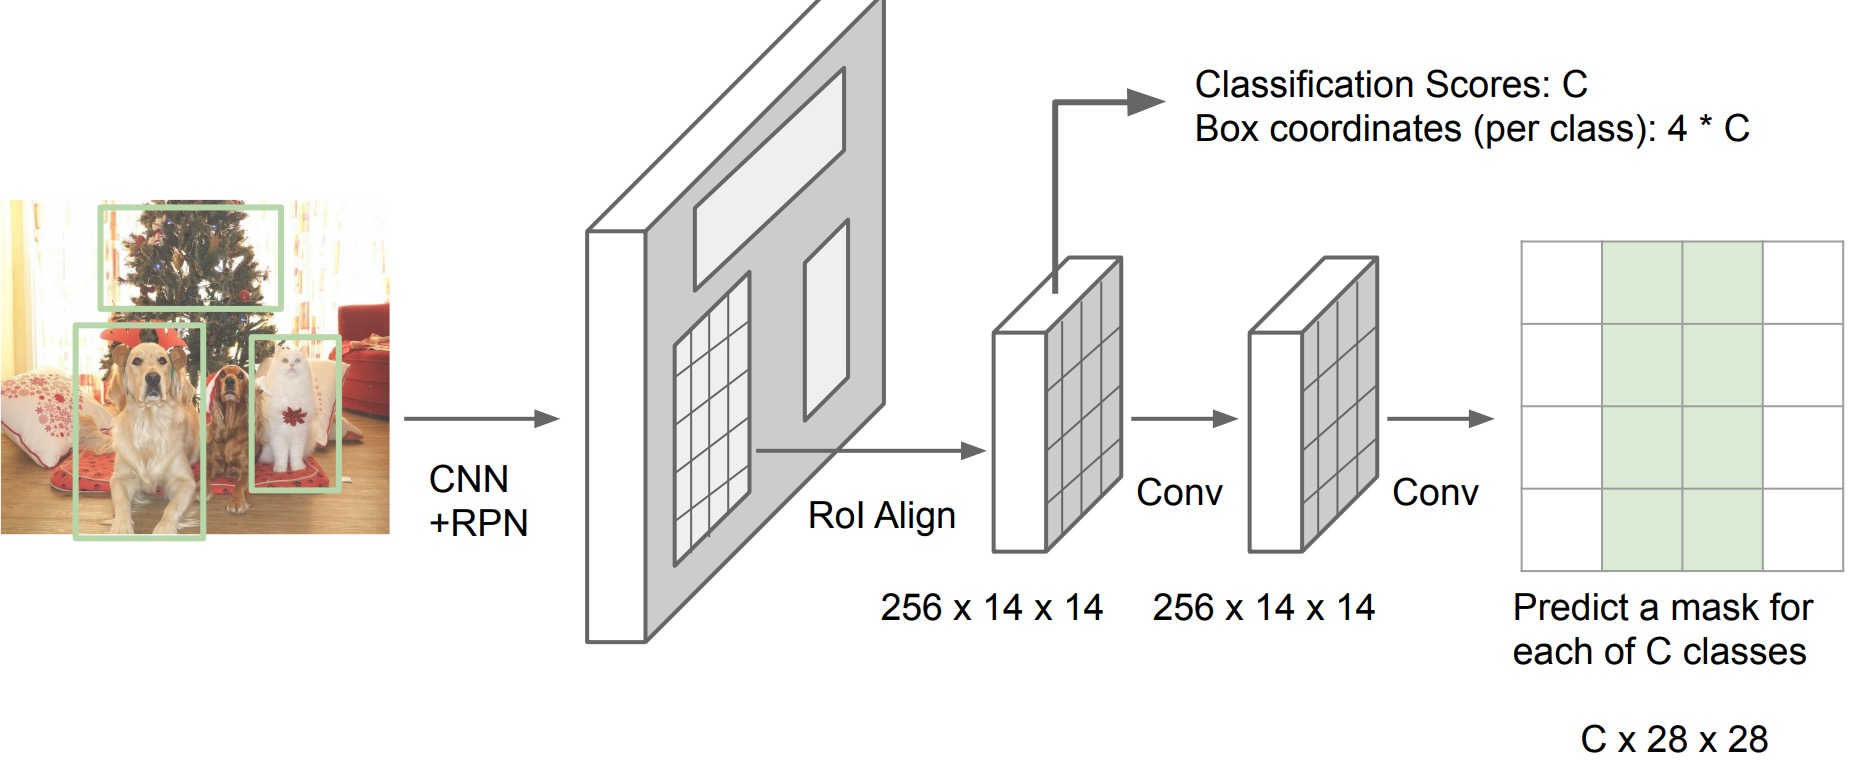
\includegraphics[width=0.8\linewidth]{figs/chapter6/Mask R-CNN.jpg}
\end{figure}

类似于之前的 Faster R-CNN，不过最后一个卷积网络不是对区域内容进行分类，而是对每一类输出一个 mask。

Mask R-CNN 还可以做 pose estimation，即预测人体的姿势。
